\section{第 13 章：引用}

\begin{taplauthorsolutionentrybox}
\phantomsection
\label{sol:author:13.1.1}
\textbf{13.1.1 解答}

\begin{center}
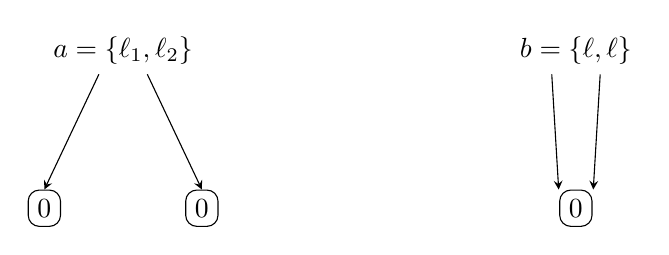
\begin{tikzpicture}[>=stealth,scale=1.25,baseline=(current bounding box.center)]
  \node (a) at (0,1.6) {\(a=\{\ell_1,\ell_2\}\)};
  \node[draw,rounded corners] (a1) at (-0.8,0) {\(0\)};
  \node[draw,rounded corners] (a2) at (0.8,0) {\(0\)};
  \draw[->] ([xshift=-7pt]a.south) -- (a1.north);
  \draw[->] ([xshift=7pt]a.south) -- (a2.north);

  \node (b) at (4.6,1.6) {\(b=\{\ell,\ell\}\)};
  \node[draw,rounded corners] (b1) at (4.6,0) {\(0\)};
  \draw[->] ([xshift=-7pt]b.south) -- ([xshift=-5pt]b1.north);
  \draw[->] ([xshift=7pt]b.south) -- ([xshift=5pt]b1.north);
\end{tikzpicture}
\end{center}

\taplsolutionbacklink{ex:13.1.1}{返回练习 13.1.1}
\end{taplauthorsolutionentrybox}

\begin{taplauthorsolutionentrybox}
\phantomsection
\label{sol:author:13.1.2}
\textbf{13.1.2 解答}

不行：现在，凡是用不同于 \(\mathit{update}\) 所接收索引的索引调用
\(\mathit{lookup}\)，都会发散。原因是，在用新函数覆盖 \(a\) 之前，必须先
取出 \(a\) 中原先保存的值；否则，等到真正执行查找时，读到的将是刚写入的
新函数，而不是原函数。

\taplsolutionbacklink{ex:13.1.2}{返回练习 13.1.2}
\end{taplauthorsolutionentrybox}

\begin{taplauthorsolutionentrybox}
\phantomsection
\label{sol:author:13.1.3}
\textbf{13.1.3 解答}

设语言提供原始操作 \(\mathsf{free}\)：它接收引用单元，释放相应存储，并且
下一个新分配的引用单元会复用同一块内存。于是程序
\begin{lstlisting}
let r = ref 0 in
let s = r in
free r;
let t = ref true in
t := false;
succ (!s)
\end{lstlisting}
会求值到卡住项 \(\mathsf{succ}\;\mathsf{false}\)。别名在这里至关重要：
即使余下表达式中不再自由出现变量 \(r\)，同一位置仍可能由别名 \(s\) 访问，
所以不能简单规定“若余下表达式中自由出现 \(r\)，则 \(\mathsf{free}\;r\)
非法”来发现无效释放。

在 C 这类手工管理内存的语言中，很容易写出同类例子；这里的
\(\mathsf{ref}\) 相当于 C 的 \texttt{malloc}，\(\mathsf{free}\) 则是 C 中
\texttt{free} 的简化版本。

\taplsolutionbacklink{ex:13.1.3}{返回练习 13.1.3}
\end{taplauthorsolutionentrybox}

\begin{taplauthorsolutionentrybox}
\phantomsection
\label{sol:author:13.3.1}
\textbf{13.3.1 解答}

垃圾收集的一种简单形式化方法如下。

\begin{enumerate}
  \item 令位置集合 \(L\) 为有限集，以此刻画内存容量有限。分配规则
    \rulename{E-RefV} 还应要求新位置 \(\ell\in L\)。把 \(L\) 限定为
    有限集并不是定义垃圾收集所必需的；这样做是为了让第 5 项中的“内存耗尽”
    成为一个需要处理的真实情形。

  \item 定义存储中的位置可达性。记 \(\mathit{locations}(t)\) 为项 \(t\)
    中提到的位置集合。若
    \(\ell'\in\mathit{locations}(\mu(\ell))\)，就说在存储 \(\mu\) 中
    \(\ell'\) 从 \(\ell\) 一步可达；若存在从 \(\ell\) 到 \(\ell'\) 的
    有限位置序列，且每个位置都从前一位置一步可达，就说 \(\ell'\) 从
    \(\ell\) 可达。最后，把存储 \(\mu\) 中从
    \(\mathit{locations}(t)\) 可达的位置集合记作
    \(\mathit{reachable}(t,\mu)\)。

  \item 用关系 \(t\mid\mu\trans_{gc}t\mid\mu'\) 描述垃圾收集：
    \[
    \inferrule*[right=\rulename{E-GC}]
      {\mu'=\mu\text{ 在 }\mathit{reachable}(t,\mu)\text{ 上的限制}}
      {t\mid\mu\trans_{gc}t\mid\mu'}
    \]
    也就是说，\(\dom(\mu')=\mathit{reachable}(t,\mu)\)，而且 \(\mu'\)
    在该定义域中的取值与 \(\mu\) 相同。

  \item 把求值序列定义为普通求值步骤与垃圾收集步骤交错组成的序列：
    \[
      \overset{gc}{\transmulti}
      \ \mathrel{\stackrel{\mathrm{def}}{=}}\ 
      (\trans\ \cup\ \trans_{gc})^*
    \]
    不能把 \rulename{E-GC} 直接加入普通的单步求值关系；垃圾收集只能在
    能看见整个待求值项的最外层执行。例如，若允许在应用左侧的求值过程中
    收集垃圾，就可能复用仍由应用右侧提到的位置，因为只看左侧时看不见这些
    位置仍然可达。

  \item 证明上述改动除了引入“内存耗尽”的可能性之外，不会改变最终结果。
    更具体地说：
    \begin{enumerate}[label=\textup{\alph*.}]
      \item 假设在有限位置集 \(L\) 上、允许垃圾收集时有
        \[
          t\mid\mu\overset{gc}{\transmulti}t'\mid\mu''
        \]
        那么，在无限存储中不使用垃圾收集时，存在存储 \(\mu'\)，使得
        \[
          t\mid\mu\transmulti t'\mid\mu',
          \qquad
          \dom(\mu'')\subseteq\dom(\mu'),
          \qquad
          \left.\mu'\right|_{\dom(\mu'')}=\mu''
        \]
        也就是说，两次执行得到同一个最终项；不带垃圾收集的存储可能保留更多
        位置，但两个存储在共同定义域上的取值相同。

      \item 反过来，假设在无限存储中不使用垃圾收集时有
        \[
          t\mid\mu\transmulti t'\mid\mu'
        \]
        那么，在有限位置集 \(L\) 上允许垃圾收集时，以下两种情况必有一种
        发生：
        \begin{enumerate}[label=\textup{\roman*.}]
          \item 存在存储 \(\mu''\)，使得
            \[
              t\mid\mu\overset{gc}{\transmulti}t'\mid\mu'',
              \qquad
              \dom(\mu'')\subseteq\dom(\mu'),
              \qquad
              \left.\mu'\right|_{\dom(\mu'')}=\mu''
            \]
            即带垃圾收集的执行也得到同一个最终项，而最终存储只保留仍然需要
            的位置；

          \item 求值在某个状态 \(t''\mid\mu''\) 耗尽内存：下一步必须分配
            新位置，但
            \[
              \mathit{reachable}(t'',\mu'')=L
            \]
            所有可用位置都仍然可达，因而没有位置可以回收或重新分配。
        \end{enumerate}
    \end{enumerate}
\end{enumerate}

\translatornote{作者官方勘误说明，原书本题第 5 项的 5a 与 5b 排写混乱：
两条命题比较的应当是“有限位置集上带垃圾收集的执行”与“无限存储中不带垃圾
收集的执行”。上文保留原书 5a、5b 的双向模拟结构，并按这项勘误明确两边的
运行环境；5b(i) 中存储一致性的范围也按勘误修正为 \(\mu''\) 的定义域。}

类型安全性还要求同步处理存储类型。若垃圾收集把 \(\mu\) 限制为
\(\mu'\)，就应把相应的存储类型 \(\Sigma\) 也限制到
\(\dom(\mu')\)；否则，原保持性陈述只允许存储类型增长，无法描述垃圾
收集删除位置之后的状态。进展性与保持性的陈述和证明都要使用这一同步限制
后的存储类型。

这种简化模型忽略了真实存储的若干方面，例如不同种类的值通常占用不同大小
的内存，以及终结器和弱指针等更高级的语言特性。操作语义中更精细的垃圾
收集处理可见 Morrisett 等人（1995）。

\taplsolutionbacklink{ex:13.3.1}{返回练习 13.3.1}
\end{taplauthorsolutionentrybox}

\Needspace{10\baselineskip}
\begin{taplauthorsolutionentrybox}
\phantomsection
\label{sol:author:13.4.1}
\textbf{13.4.1 解答}

\begin{lstlisting}
let r1 = ref (lambda x:Nat. 0) in
let r2 = ref (lambda x:Nat. (!r1) x) in
(r1 := (lambda x:Nat. (!r2) x);
 r2)
\end{lstlisting}

\taplsolutionbacklink{ex:13.4.1}{返回练习 13.4.1}
\end{taplauthorsolutionentrybox}

\begin{taplauthorsolutionentrybox}
\phantomsection
\label{sol:author:13.5.2}
\textbf{13.5.2 解答}

设 \(\mu\) 是只有一个位置 \(\ell\) 的存储：
\[
  \mu=(\ell\mapsto\lambda x:\tapltype{Unit}.\,(!\ell)\,x)
\]
并令 \(\Gamma\) 为空上下文。则 \(\mu\) 对以下两个存储类型都是良类型的：
\[
\begin{aligned}
\Sigma_1&=\ell:\tapltype{Unit}\to\tapltype{Unit},\\
\Sigma_2&=\ell:\tapltype{Unit}\to
  (\tapltype{Unit}\to\tapltype{Unit})
\end{aligned}
\]

\taplsolutionbacklink{ex:13.5.2}{返回练习 13.5.2}
\end{taplauthorsolutionentrybox}

\begin{taplauthorsolutionentrybox}
\phantomsection
\label{sol:author:13.5.8}
\textbf{13.5.8 解答}

这个系统中存在不能规范化的良类型项。练习 13.1.2 已经给出一例。还有一例是
\[
\begin{aligned}
t_1={}&\lambda r:\tapltype{Ref}
  (\tapltype{Unit}\to\tapltype{Unit}).\,
  \bigl(r:=\lambda x:\tapltype{Unit}.\,(!r)\,x;\,(!r)\;\mathsf{unit}\bigr),\\
t_2={}&\mathsf{ref}\,(\lambda x:\tapltype{Unit}.\,x)
\end{aligned}
\]
把 \(t_1\) 应用于 \(t_2\)，会得到一个发散的良类型项。

更一般地，可以按以下步骤借助引用定义任意递归函数；某些函数式语言实现确实
使用这种技术。

\begin{enumerate}
  \item 分配引用单元，并用适当类型的占位函数初始化：
    \begin{lstlisting}[mathescape=true]
factref = ref (lambda _:Nat. 0);
$\blacktriangleright$ factref : Ref (Nat -> Nat)
    \end{lstlisting}

  \item 定义所需函数的主体，通过引用单元的内容进行递归调用：
    \begin{lstlisting}[mathescape=true]
factbody =
  lambda n:Nat.
    if iszero n then 1 else times n ((!factref) (pred n));
$\blacktriangleright$ factbody : Nat -> Nat
    \end{lstlisting}

  \item 把真正的函数体“回填”到引用单元：
    \begin{lstlisting}
factref := factbody;
    \end{lstlisting}

  \item 取出引用单元的内容并使用：
    \begin{lstlisting}[mathescape=true]
fact = !factref;
fact 5;
$\blacktriangleright$ 120 : Nat
    \end{lstlisting}
\end{enumerate}

\taplsolutionbacklink{ex:13.5.8}{返回练习 13.5.8}
\end{taplauthorsolutionentrybox}
